\chapter{Implementation}\label{ch:implementation}\glsresetall
% Python
% Data collection - ccxt, binance, coinmarketcap
% historica data - anomaly detection - matplotlib -ohlcv - pandas - numpy 
% labeling - matplotlib - ohlcv - anomaly d
% generating dataset

%XXX Since design will focus on each component, this section can mirror the previous chapter, but instead of high level overview, describe how you implemented the description from the design chapter, programming language, libraries etc.


\section{Data Collection}

\section{Labeling}
\begin{figure}
    \centering
    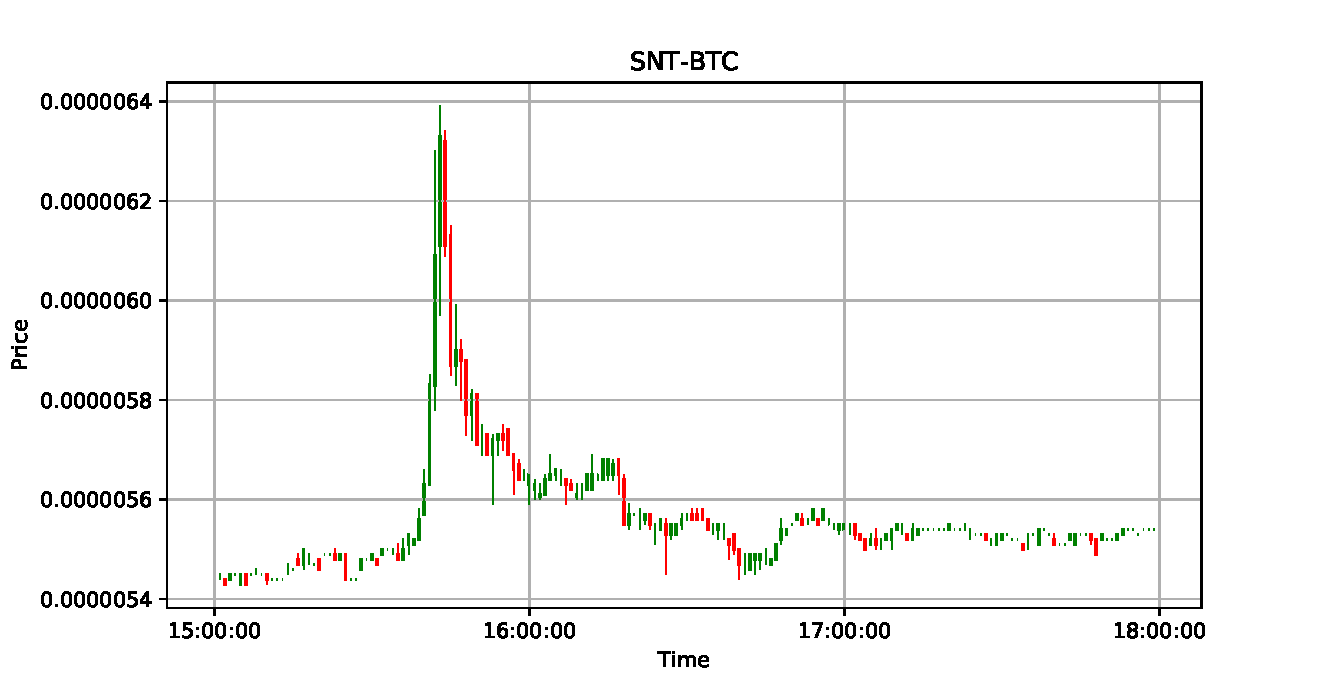
\includegraphics[width=\textwidth]{true_1.pdf}
    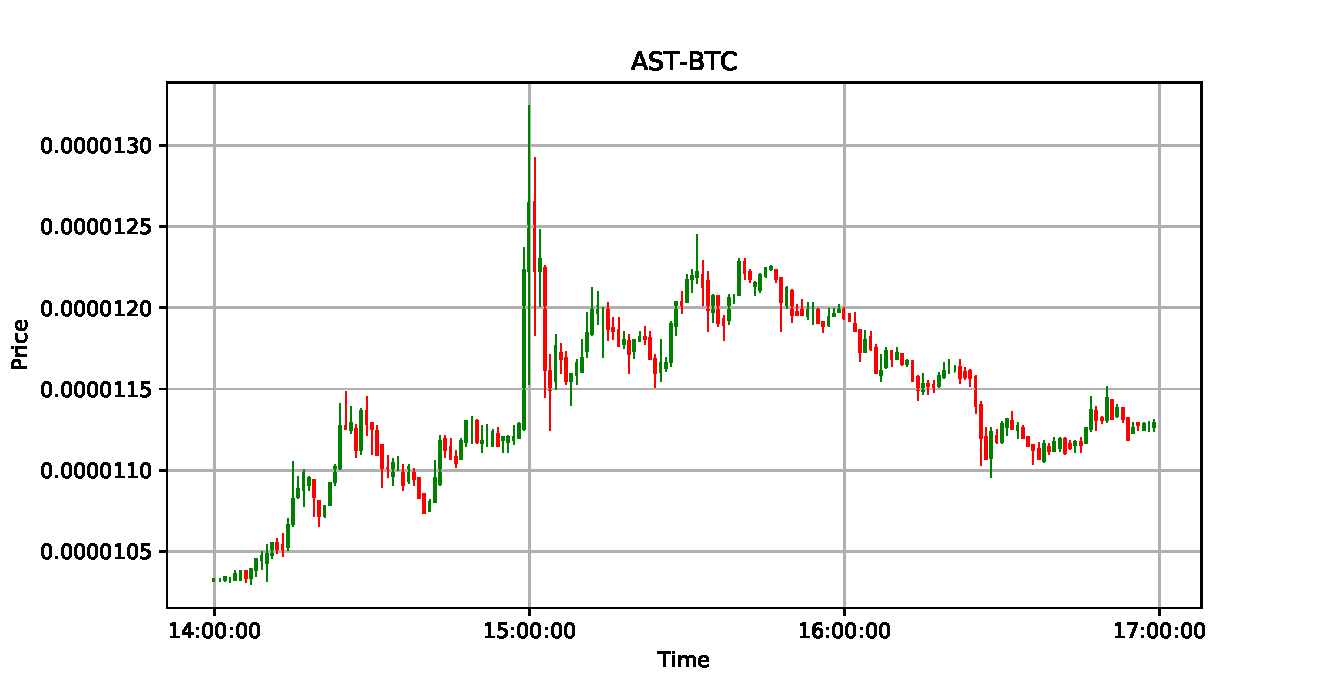
\includegraphics[width=\textwidth]{true_2.pdf}
    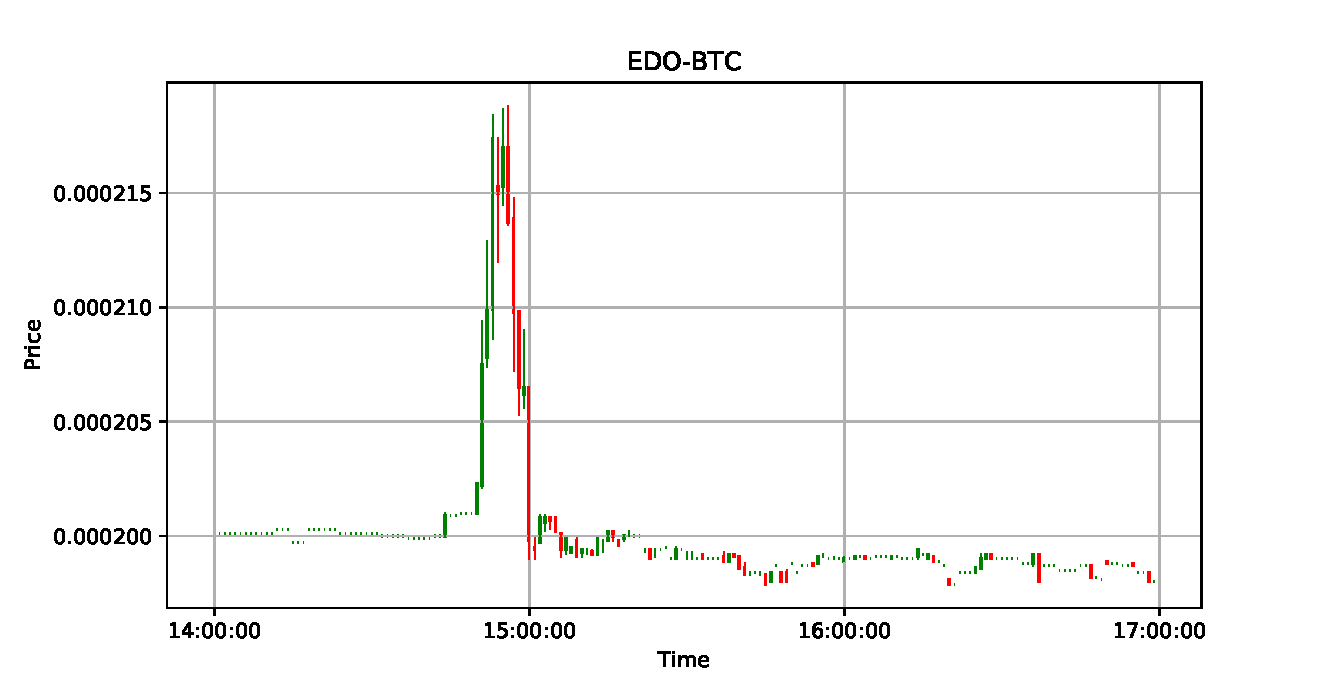
\includegraphics[width=\textwidth]{true_3.pdf}
    \caption{True}
    \label{fig:label_true}
\end{figure}

\begin{figure}
    \centering
    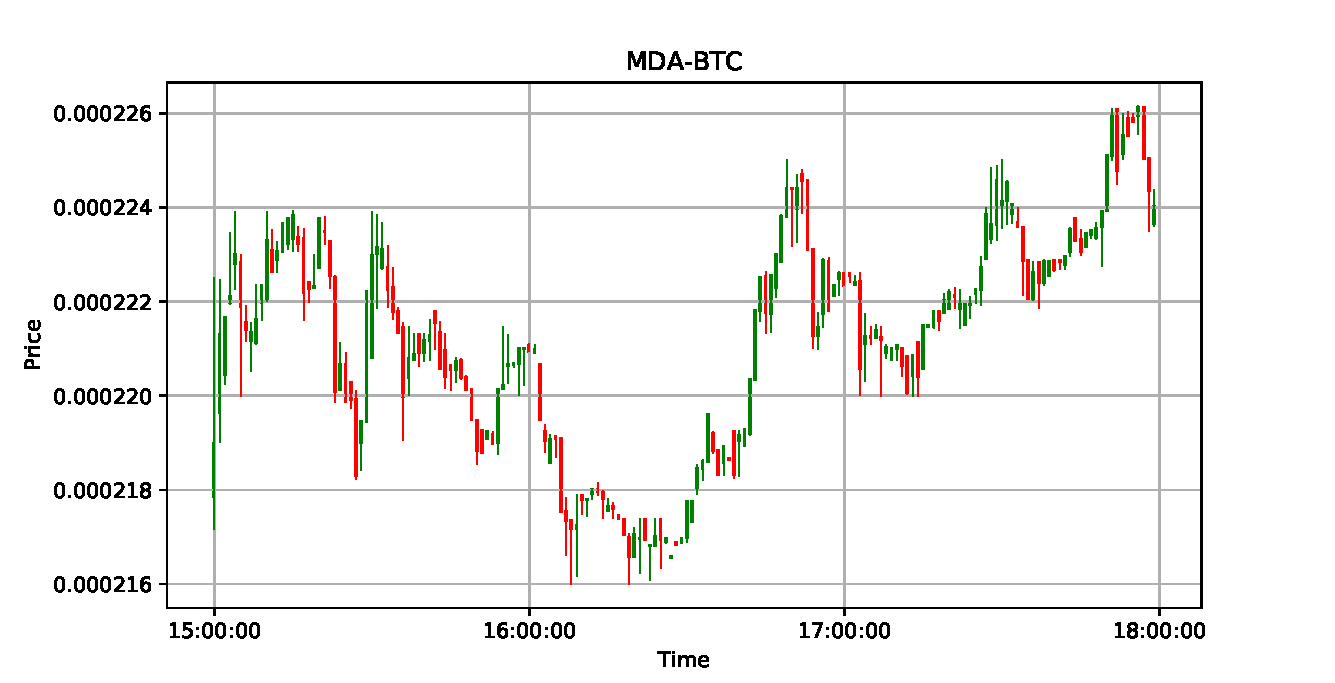
\includegraphics[width=\textwidth]{false_1.pdf}
    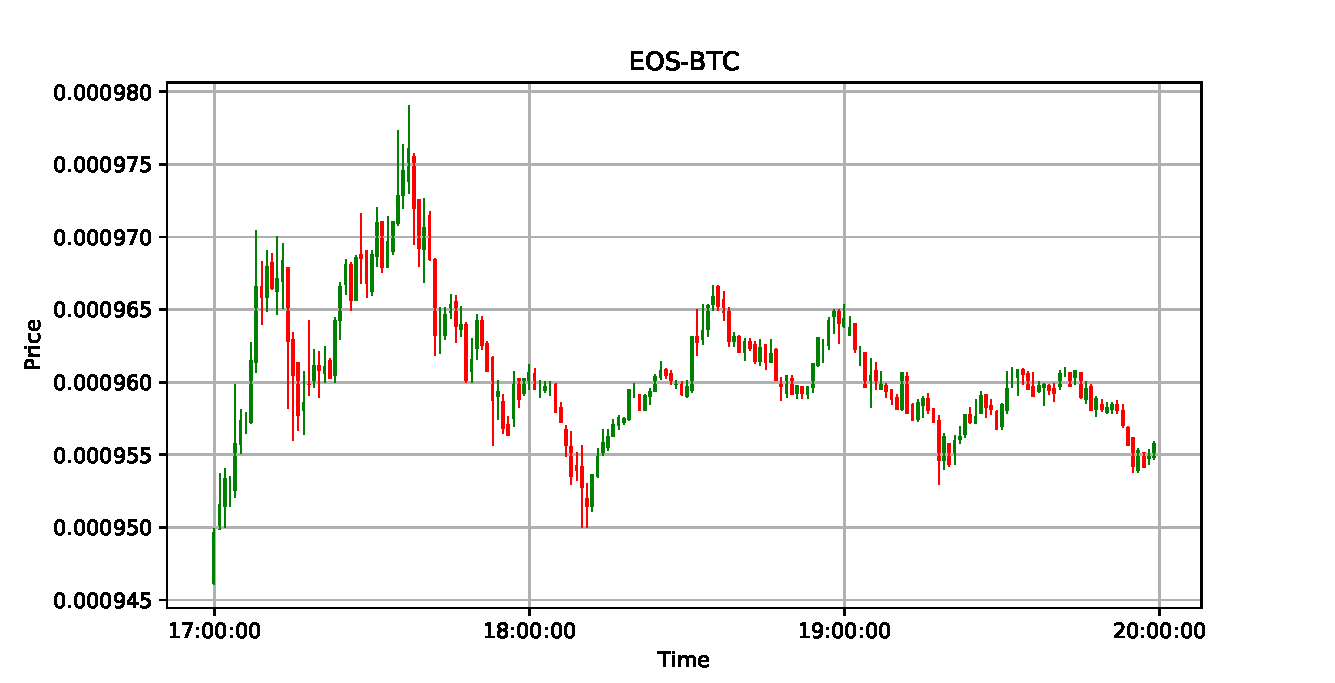
\includegraphics[width=\textwidth]{false_2.pdf}
    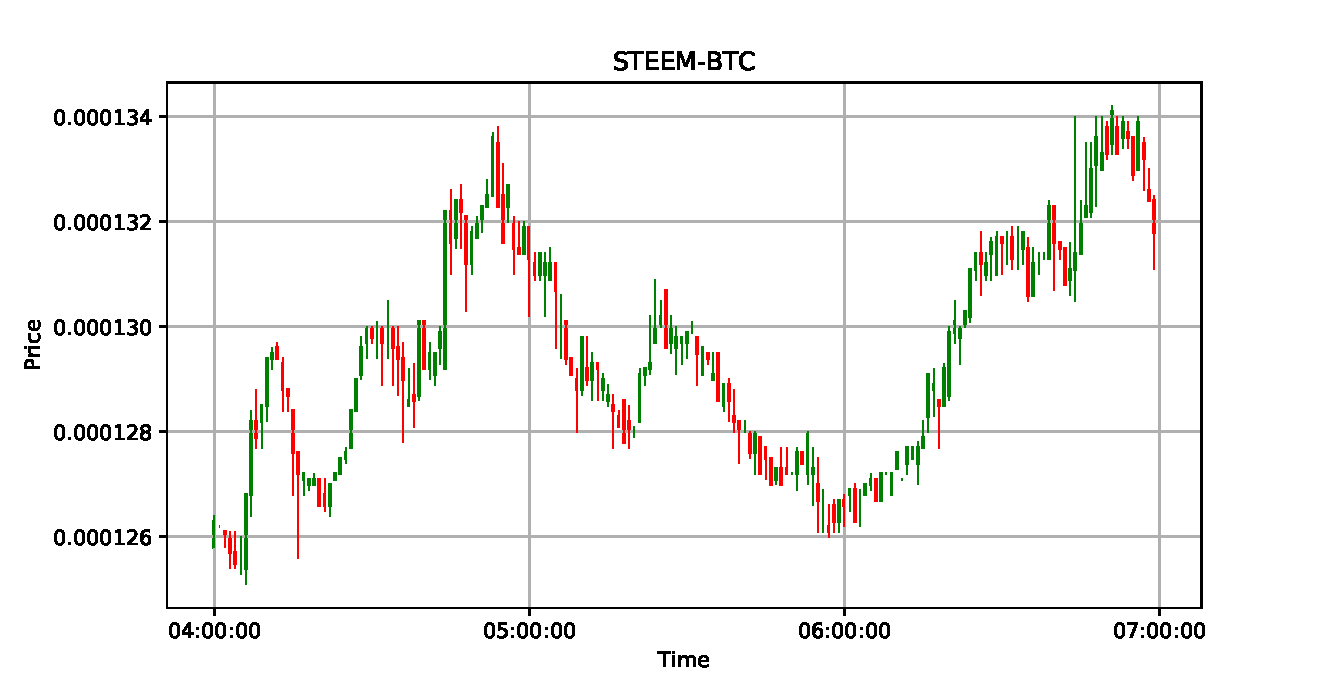
\includegraphics[width=\textwidth]{false_3.pdf}
    \caption{False}
    \label{fig:label_false}
\end{figure}